\setAuthor{}
\setRound{piirkonnavoor}
\setYear{2019}
\setNumber{G 10}
\setDifficulty{10}
\setTopic{TODO}

\prob{3 dioodi}
Joonisel näidatud skeem sisaldab kahte ühesugust takistit ($r=\SI {1.0}\ohm$) ning kolme valgusdioodi: sinist, rohelist ja punast, mis on tähistatud vastavalt tähtedega $S$, $R$ ja $P$. Dioodide voolutugevuse sõltuvuse pingest võib lugeda lihtsuse mõttes selliseks nagu näidatud kõrvaloleval graafikul: voolutugevus on null, kui dioodile rakendatud päripinge on väiksem avanemispingest $V_a$ ning suvalise nullist erineva pärivoolu korral on dioodi pinge võrdne $V_a$-ga. Avanemispinged on dioodidel järgmised: sinisel $\SI{3.2}V$, rohelisel  $\SI{2.6}V$ ja punasel  $\SI{1.8}V$. Sisendklemmidele $A$ ja $B$ rakendatakse konstantse voolu allikas, mis hoiab klemmi $A$ siseneva ning klemmist $B$ väljuva voolu võrdse $I=\SI{1.0}A$-ga. Millist võimsust tarbivad dioodid (näidata ära iga dioodi võimsus eraldi)? 
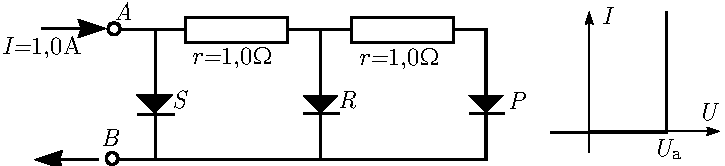
\includegraphics[scale=0.8]{2019-v2g-10-yl.pdf}

\hint

\solu
Lahendus. Vaatleme protsessi, kus sisendpinget hakatakse aeglaselt suurendama alates nullist. Väikese voolu korral on pingelang takisteil tühine, seetõttu on kõigi dioodide pinged peaaegu võrdsed. See tähendab, et esimesena avaneb kõige madalama avanemispingega diood - punane diood. Voolu kasvatamisel pingelang takisteil kasvab; et esialgu on roheline diood suletud, siis läbib mõlemat takistid sama tugev vool, mis tähendab et ka takistite pinged on võrdsed. Et rohelise ja punase dioodi avanemispingete vahe on suurem, kui sinise ja rohelise dioodi avanemispingete vahe, siis järgmisena avaneb sinine diood. Sellest hetkest, kui sinine diood on avatud, ei saa takistite voolud enam kasvada (potentsiaalid takistite otstel on määratud sinise ja punase dioodi avanemispingetega) mistõttu roheline diood jääb kogu aeg suletuks, st rohelisse dioodi minev vool on null \pp{3}. Nüüd on kaks takistit järjestikühenduses, kusjuures pinge otste vahel on võrdne sinise ja punase dioodi avanemispingete vahega $U_T=\SI{1.4}V$. \pp{2} See tähendab, et vool takisteis on $I_t=U_t/(2r)=\SI{0.7}A$ \pp{2}. See on ka punase dioodi vool, mis tähendab, et punase dioodi võimsus $P_p=\SI{0.7}A\cdot \SI{1.8}V\approx {1.3}W$ \pp{1}. Sinisesse dioodi läheb sisendvoolu ja takistite voolu vahe $\SI{0.3}A$ \pp{2}, mistõttu sinise dioodi võimsus $P_s=\SI{0.3}A\cdot \SI{3.2}V\approx {1.0}W$ \pp{1}. Rohelise dioodi võimsus on null. \pp{1}
\probend